\chapter{Simulating the Lyman-alpha forest: The Sherwood simulation suite} \label{chap:sherwood}

\section{Prelude on cosmological simulation}

\section{Obtaining mock Lyman-alpha skewers from cosmological simulations}

\section{Statistical analysis of the effect of dark matter in the flux and density fields}


\begin{figure}
        \centering
            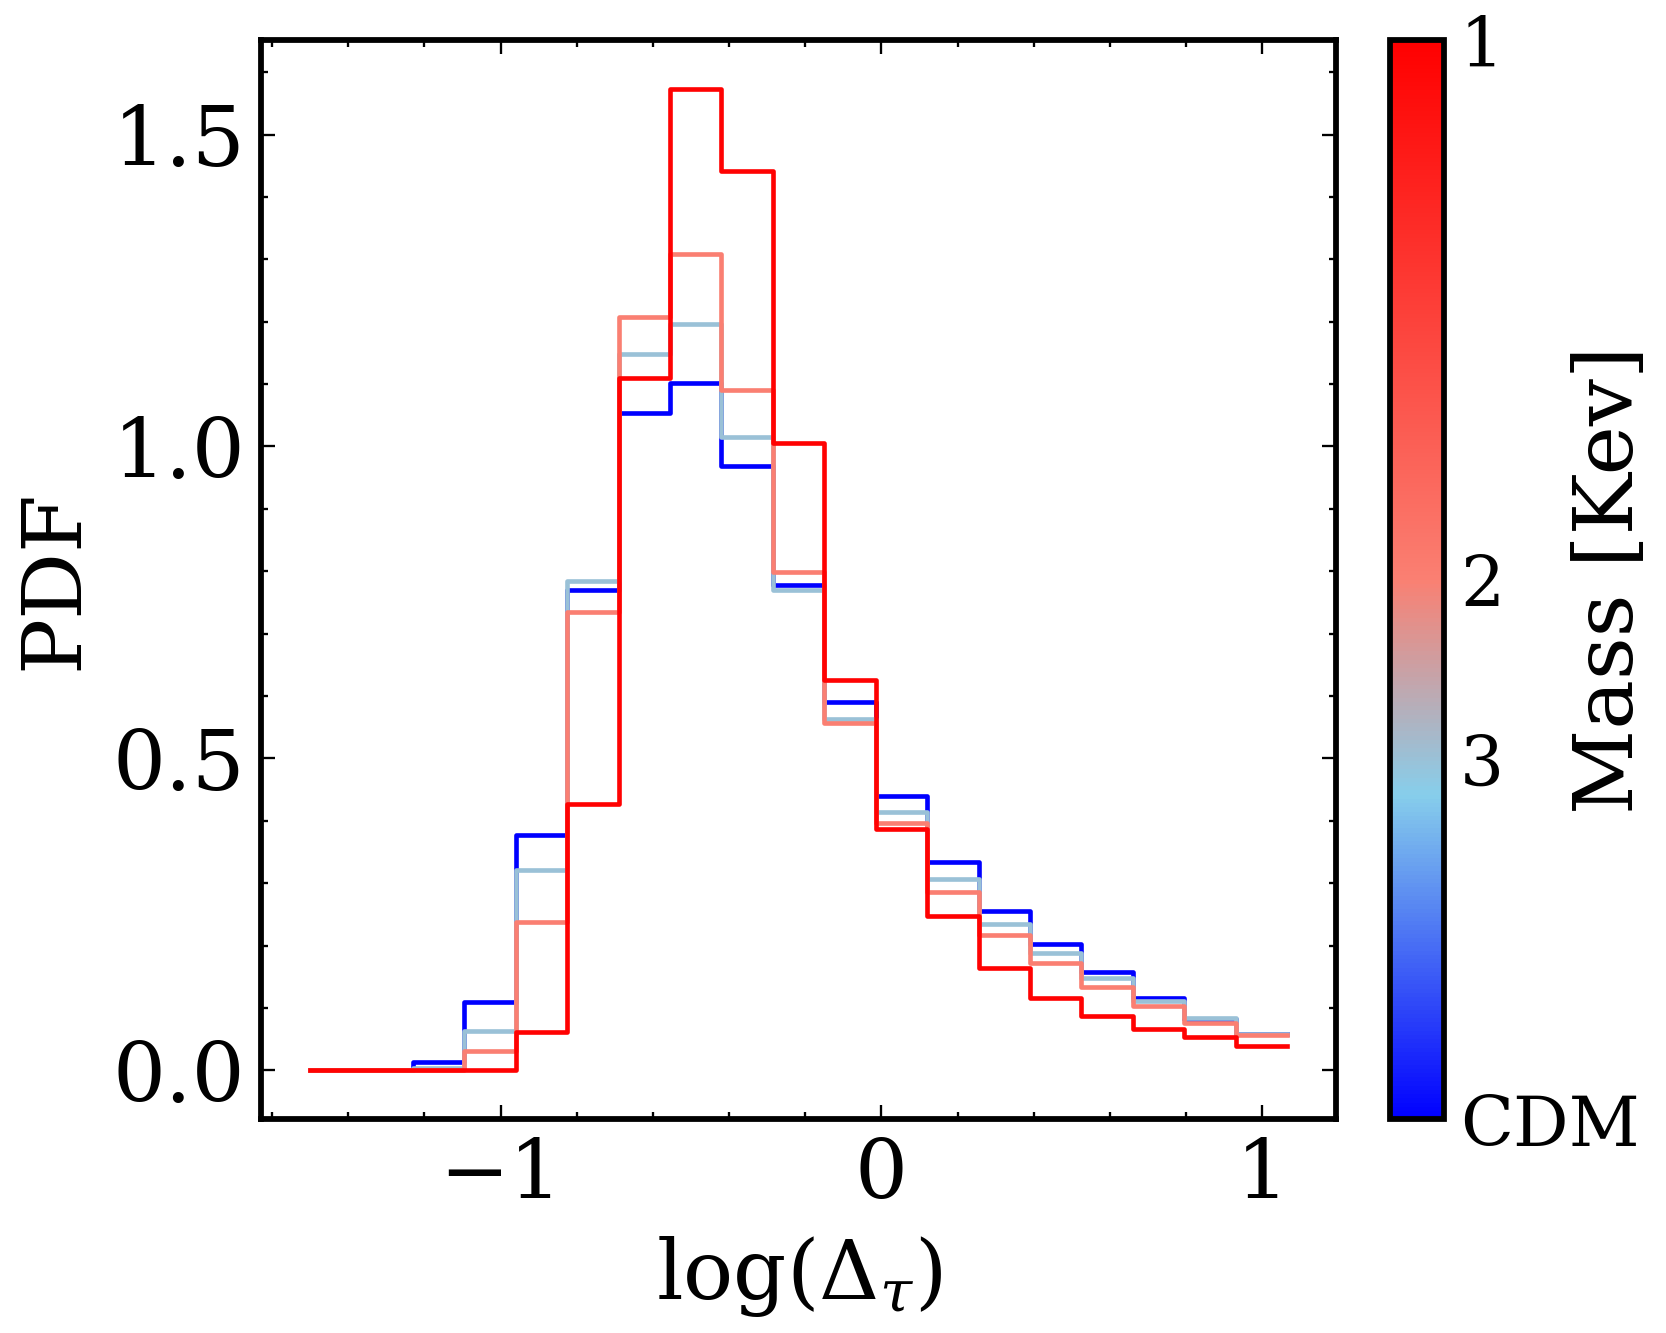
\includegraphics[width=0.8\textwidth]{img/ML/pdf_density_sherwood.png}
            \caption{The $\Delta_\tau$ probability distriburion function (PDF) for different WDM models in the \texttt{SHERWOOD} suite.}
            \label{fig: exact density PDF}
\end{figure}
    
\begin{figure}
        \centering
        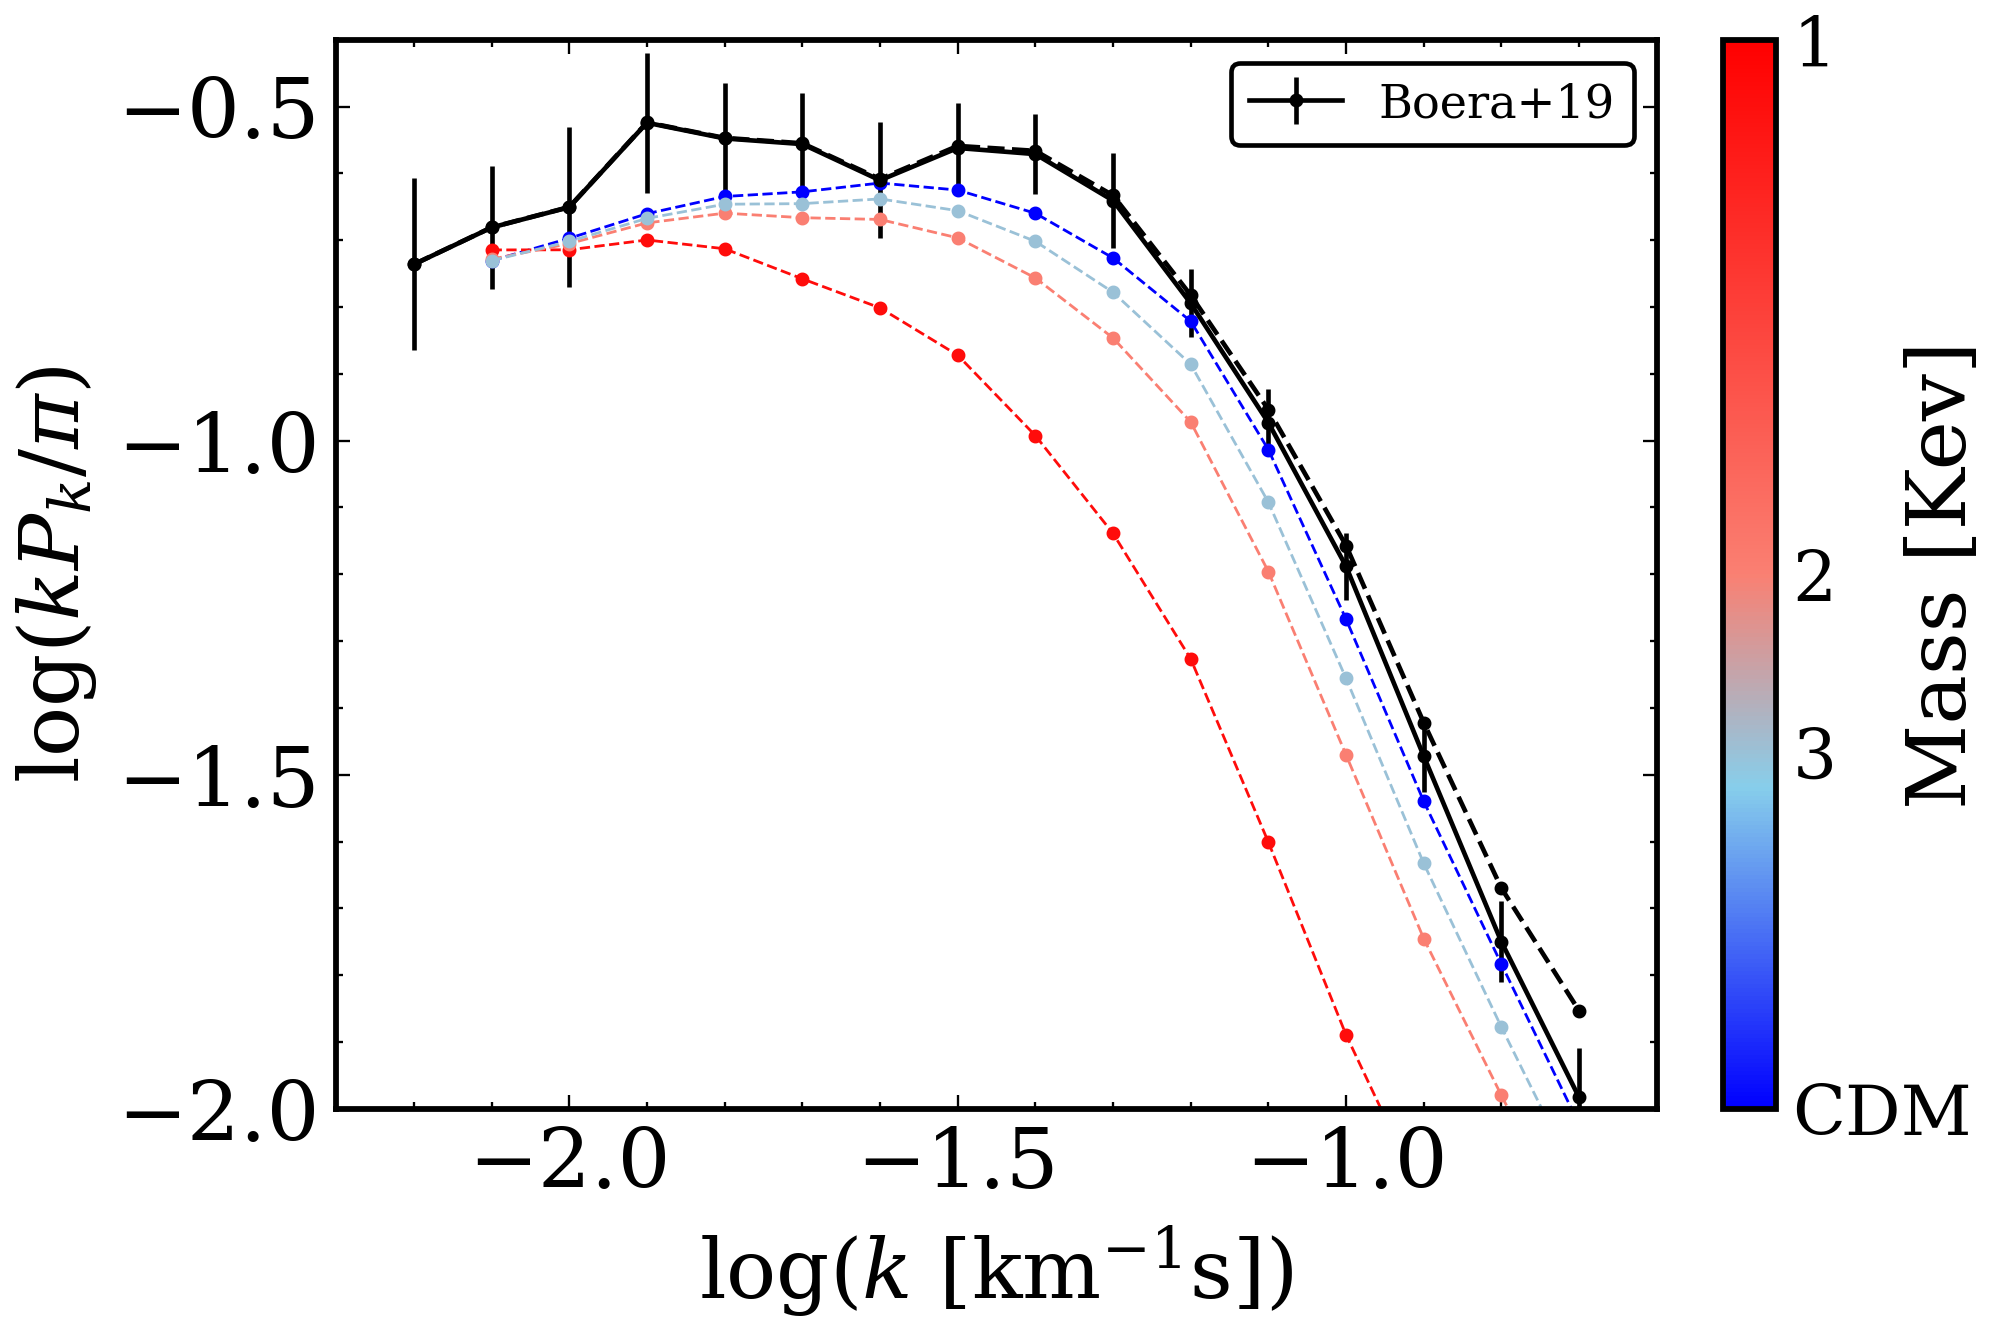
\includegraphics[width=0.8\textwidth]{img/ML/PS_sherwood.png}
        \caption{The Lyman-$\alpha$ flux power spectrum for different WDM models in the \texttt{SHERWOOD} simulation suite. For reference, we also plot the observed PS by \cite{Boera_2019}.}
        \label{fig: sherwood exact PS}     
\end{figure}


DISCUSS plots with color bar of pdf and ps of Density discuss the boeara discrepancy




\section{Peculiar velocities and optical depth-weighted quantities}\label{sec: optical depth weighted}